\documentclass[11pt,a4paper]{article}

% Datos de la actividad
\newcommand{\codigoactividad}{PE-U1}
\newcommand{\nombreactividad}{Comunicación entre procesos con sockets TCP y gRPC}
\newcommand{\integrantes}{Castro Coello Mario Sebastián \\ Loor Suárez Steffanny del Rocío \\ Quintero Rico Luis David \\ Rivas Piloso Dayver Yahir}
\newcommand{\repositorio}{https://github.com/reyshadow0/isr701-pe-u1}
\newcommand{\fechaentrega}{18 de noviembre de 2026}

\usepackage[T1]{fontenc}
\usepackage[utf8]{inputenc}
\usepackage[spanish,es-tabla,es-nodecimaldot]{babel}
\usepackage{lmodern}
\usepackage{microtype}
\usepackage[a4paper,margin=2.5cm]{geometry}
\usepackage{graphicx}
\usepackage{booktabs}
\usepackage{tabularx}
\usepackage{longtable}
\usepackage{array}
\usepackage{float}
\usepackage{xcolor}
\usepackage{amsmath}
\usepackage{tikz}
\usetikzlibrary{arrows.meta,positioning,fit,backgrounds}
\usepackage{listings}
\usepackage{csquotes}
\usepackage[backend=biber,style=ieee]{biblatex}
\addbibresource{referencias.bib}
\usepackage[hidelinks]{hyperref}

\graphicspath{{figuras/}}

% Permite cortar URL largas en la bibliografía (evita desbordes)
\setcounter{biburlnumpenalty}{100}
\setcounter{biburlucpenalty}{100}
\setcounter{biburllcpenalty}{100}

\lstset{
  basicstyle=\ttfamily\small,
  breaklines=true,
  frame=single,
  numbers=left,
  numberstyle=\tiny,
  showstringspaces=false,
  extendedchars=true,
  literate={á}{{\'a}}1 {é}{{\'e}}1 {í}{{\'i}}1 {ó}{{\'o}}1 {ú}{{\'u}}1
           {Á}{{\'A}}1 {É}{{\'E}}1 {Í}{{\'I}}1 {Ó}{{\'O}}1 {Ú}{{\'U}}1
           {ñ}{{\~n}}1 {Ñ}{{\~N}}1 {ü}{{\"u}}1 {¿}{{?`}}1 {¡}{{!`}}1
}
\renewcommand{\lstlistingname}{Código}

\hypersetup{pdftitle={\codigoactividad: \nombreactividad}}

\begin{document}

\begin{titlepage}
  \centering
  {\large\bfseries UNIVERSIDAD TÉCNICA ESTATAL DE QUEVEDO\par}
  \vspace{0.3cm}
  {Facultad de Ciencias de la Computación\par}
  {Carrera de Software\par}
  \vspace{2.5cm}
  {\large Aplicaciones Distribuidas (ISR-701)\par}
  \vspace{1.5cm}
  {\Large\bfseries \codigoactividad\par}
  \vspace{0.4cm}
  {\LARGE \nombreactividad\par}
  \vspace{1cm}
  {\large Práctica experimental de la Unidad 1\par}
  \vfill
  \begin{tabular}{@{}rl@{}}
    \textbf{Integrantes:}      & \begin{tabular}[t]{@{}l@{}}\integrantes\end{tabular} \\[2pt]
    \textbf{Docente:}          & Gleiston Cicerón Guerrero Ulloa, PhD \\
    \textbf{Nivel / paralelo:} & Séptimo nivel / B \\
    \textbf{Periodo:}          & SPA 2026--2027 \\
    \textbf{Fecha:}            & \fechaentrega \\
  \end{tabular}
  \par\vspace{1cm}
  {\small Repositorio: \url{\repositorio}\par}
\end{titlepage}

\tableofcontents
\newpage

\section{Objetivo e hipótesis}
\subsection{Objetivo}

Comparar la latencia de ida y vuelta (mediana y percentil~95) y los mensajes por segundo de sockets TCP con JSON y de gRPC con Protocol Buffers, en tres nodos que corren como procesos en \emph{localhost}, con mensajes de unos 100~bytes y de unos 10~KB y con uno o tres clientes enviando a la vez. Verificar, además, con los registros de los 20 intercambios, que los relojes de Lamport cumplen sus reglas en los dos mecanismos, y medir cómo cambia su tiempo de convergencia al pasar de 2 a 3 y a 4 nodos.

\subsection{Hipótesis}

Las hipótesis se escribieron antes de la corrida oficial. Suponen que cada cliente abre una sola conexión TCP o un solo canal de gRPC y hace por ahí sus 100 envíos, de modo que el saludo inicial de TCP y de HTTP/2 queda fuera de la medición. Los dos mecanismos corren en la misma máquina, con Python~3.13, y nunca a la vez.

En \emph{localhost} casi no hay red, por eso esperamos que la diferencia entre los dos mecanismos salga sobre todo del software que procesa cada mensaje. Con sockets, el cliente convierte el mensaje a JSON y lo envía con un salto de línea al final; el servidor lo lee, lo vuelve a convertir y responde con un acuse, también en JSON. Encima de TCP no hay otra capa. Con gRPC, cada llamada serializa el mensaje en binario, lo mete en tramas de HTTP/2 con sus encabezados y pasa por las capas de la biblioteca: los metadatos, el plazo de la llamada y el hilo del \texttt{ThreadPoolExecutor} que la atiende en el servidor.

Las dos fuentes que siguen no miden este mismo caso y se usan como evidencia indirecta. Zhu \emph{et al.}~\cite{Zhu2023} midieron el proxy Envoy, escrito en C++, con mensajes de 100~bytes: cuando procesaba el tráfico como gRPC añadía unas cinco veces más latencia que cuando lo trataba como TCP, y la mayor parte de ese costo extra venía de interpretar el protocolo. Es otro programa y otro lenguaje, pero muestra que las capas de gRPC tienen un costo por mensaje que TCP no paga. Niswar \emph{et al.}~\cite{Niswar2024} compararon gRPC con REST y con GraphQL, que usaban HTTP/1.1. gRPC tuvo menor tiempo de respuesta en la mayoría de sus pruebas, aunque en la de 100 solicitudes concurrentes con datos anidados REST fue más rápido. En ese estudio las otras opciones también cargan con HTTP. Aquí sockets no lo usa, por eso no esperamos que la ventaja de gRPC frente a REST se repita frente a sockets.

Con 100~bytes esperamos que pese sobre todo el costo fijo de cada llamada. Con 10~KB, el mensaje es en su mayor parte texto, y un texto ASCII ocupa casi lo mismo en los dos formatos: con nuestros campos, JSON suma unos 40~bytes más que Protocol Buffers por los nombres de los campos y las comillas. Eso es cerca del 40\,\% de un mensaje de 100~bytes y menos del 1\,\% de uno de 10~KB. Si el texto lleva tildes o eñes, JSON escribe cada una como \texttt{\textbackslash uXXXX} y la diferencia crece. Copiar y convertir esos 10~KB cuesta parecido en los dos mecanismos, de modo que la diferencia en milisegundos debería mantenerse y pesar menos frente al total.

Con tres clientes, los dos servidores atienden con hilos. En la versión estándar de CPython~3.13 solo un hilo a la vez ejecuta código Python, por el GIL. En gRPC, la red y HTTP/2 corren en el núcleo de la biblioteca, escrito en C, pero el método del servicio corre en un hilo de Python. No tenemos una fuente que diga cuál de los dos servidores sufre más esa espera. Suponemos que gRPC, porque cada llamada pasa también por código Python de la biblioteca antes y después del método. H3 pone a prueba esa suposición.

Los relojes de Lamport no llegan a un valor común, porque cada uno solo avanza. Por eso tomamos como convergencia el momento en que todos los nodos ya recibieron, directa o indirectamente, información de todos los demás, es decir, cuando en la historia causal de cada nodo hay al menos un evento de cada uno de los otros. El tiempo de convergencia va desde el primer envío de la corrida hasta la recepción con la que el último nodo cumple esa condición. Se calcula con la hora real de los registros, que se puede comparar entre nodos porque todos corren en la misma máquina y leen el mismo reloj. También contamos cuántos intercambios hicieron falta.

Los intercambios siguen una ronda en orden: el primer nodo envía al segundo, el segundo envía al tercero cuando recibe, y el último envía al primero. La ronda se repite hasta completar los 20 intercambios y sirve igual para 2, 3 y 4 nodos. Si se sigue mensaje por mensaje, todos los nodos saben de todos en el intercambio 2, 4 y 6, respectivamente, es decir, $2n-2$ para $n$ nodos. Como el patrón es fijo, ese número sale igual en todas las corridas, y las repeticiones solo aportan la variación del tiempo. Se hacen cinco corridas con cada cantidad de nodos y cada mecanismo.

\begin{description}
  \item[H1 (100~bytes, un cliente).] Sockets tiene menor mediana y menor percentil~95 de la latencia de ida y vuelta que gRPC, y más mensajes por segundo.
  \item[H2 (10~KB, un cliente).] Sockets sigue con menor mediana que gRPC, pero su ventaja relativa es menor que con 100~bytes. No esperamos que se invierta.
  \item[H3 (tres clientes a la vez, 100~bytes).] Frente a un cliente con 100~bytes, la ventaja relativa de sockets crece. Sockets mantiene menor mediana y menor percentil~95.
  \item[H4 (Lamport con 2, 3 y 4 nodos).] El tiempo de convergencia y el número de intercambios que necesita crecen al pasar de 2 a 3 y a 4 nodos, porque con más nodos la información de cada uno necesita más saltos para llegar a todos. Con la ronda esperamos 2, 4 y 6 intercambios.
\end{description}

\subsection{Criterio de decisión}

La unidad de análisis es cada repetición de 100 envíos, sin contar la de calentamiento. Por repetición, el script calcula la mediana y el percentil~95 de la latencia y los mensajes por segundo, que son los envíos de la repetición divididos entre su duración. Con tres clientes se juntan los 300 envíos de la repetición. Así quedan cinco valores por métrica, mecanismo y condición.

Hay diferencia real entre los dos mecanismos en una métrica solo si los rangos de sus cinco valores no se traslapan. Si se traslapan, no se puede afirmar que haya diferencia, y esa parte de la hipótesis no queda confirmada. H1 se cumple si las tres métricas muestran diferencia real a favor de sockets.

Para H2 y H3 no se emparejan repeticiones, así que el método sirve tanto si sockets y gRPC corren en bloques como si se intercalan. En cada condición se calculan los 25 cocientes posibles entre una de las cinco medianas de gRPC y una de las cinco de sockets. La ventaja relativa de sockets es menor con 10~KB si todos los cocientes con 10~KB quedan por debajo de todos los de 100~bytes, y crece con tres clientes si todos los cocientes con tres clientes quedan por encima de todos los de un cliente. Si los dos grupos de cocientes se traslapan, no se puede afirmar que la ventaja cambió.

H4 se cumple si, en cada mecanismo, los cinco tiempos de convergencia con 3 nodos quedan por encima de los cinco con 2, los de 4 por encima de los de 3, y el número de intercambios crece de 2 a 3 y a 4 nodos. Una corrida que no converge dentro de los 20 intercambios cuenta como mayor que cualquiera que sí convergió. Si el número de intercambios no da 2, 4 y 6, la ronda no se ejecutó como se describe aquí y hay que revisarla antes de discutir H4.


\section{Arquitectura}
\subsection{Diagrama de arquitectura}

La arquitectura que se ha desarrollado permite comparar la comunicación
entre procesos mediante sockets TCP y gRPC, cada nodo se ejecuta
como un proceso independiente y dispone de un cliente, un servidor
y un reloj lógico de Lamport compartido entre sus componentes.

Los nodos se ejecutan en el entorno local (\texttt{localhost}),
utilizando los puertos 5000, 5001, 5002 y 5003, los tres primeros
participan en el escenario principal, mientras que el cuarto
se incorpora cuando se realizan pruebas con cuatro nodos.

Esta misma arquitectura se utiliza para evaluar ambos mecanismos
de comunicación, pero las ejecuciones de TCP y gRPC se realizan
por separado, lo cual permite comparar su comportamiento sin
mantener ambos mecanismos activos simultáneamente.

\begin{figure}[H]
    \centering
    \resizebox{\textwidth}{!}{%
        % Arquitectura de comunicación distribuida: TCP y gRPC
% Requiere \usepackage{tikz} y \usetikzlibrary{arrows.meta,positioning,fit}
\shorthandoff{<>}
\begin{tikzpicture}[
    >=Stealth,
    font=\scriptsize,
    nodo/.style={
        draw,
        rounded corners=3pt,
        thick,
        minimum width=4.2cm,
        minimum height=2.0cm,
        align=center,
        fill=white
    },
    enlace/.style={thick, {Stealth}-{Stealth}},
    opcional/.style={thick, dashed, {Stealth}-{Stealth}}
]

\node[nodo] (A) at (0,0) {
    \textbf{Nodo A}\\
    \texttt{localhost:5000}\\[3pt]
    Cliente\\
    Servidor\\
    Reloj de Lamport compartido
};

\node[nodo] (B) at (8,0) {
    \textbf{Nodo B}\\
    \texttt{localhost:5001}\\[3pt]
    Cliente\\
    Servidor\\
    Reloj de Lamport compartido
};

\node[nodo] (C) at (0,-5) {
    \textbf{Nodo C}\\
    \texttt{localhost:5002}\\[3pt]
    Cliente\\
    Servidor\\
    Reloj de Lamport compartido
};

\node[nodo] (D) at (8,-5) {
    \textbf{Nodo D}\\
    \texttt{localhost:5003}\\[3pt]
    Cliente\\
    Servidor\\
    Reloj de Lamport compartido\\
    \emph{Solo escenario de 4 nodos}
};

\draw[enlace] (A.east) --
    node[above, align=center] {TCP / gRPC\\(ejecuciones separadas)}
    (B.west);

\draw[enlace] (A.south) --
    node[right, pos=0.5, xshift=2mm, align=center]
    {TCP / gRPC\\(ejecuciones separadas)}
    (C.north);

\draw[enlace] (B.south west) --
    node[right, pos=0.55, align=center] {TCP / gRPC\\(ejecuciones separadas)}
    (C.north east);

\draw[opcional] (C.east) --
    node[below, align=center] {Escenario de 4 nodos\\TCP / gRPC}
    (D.west);

\begin{scope}[on background layer]
    \node[
        draw,
        dashed,
        rounded corners=5pt,
        inner sep=12pt,
        fit=(A)(B)(C)(D),
        label={[font=\small]above:Entorno local (localhost)}
    ] {};
\end{scope}

\end{tikzpicture}
\shorthandon{<>}
    }
    \caption{Arquitectura de comunicación entre procesos mediante TCP y gRPC. Fuente: Elaboración propia}
    \label{fig:arquitectura-pe-u1}
\end{figure}

En la Figura~\ref{fig:arquitectura-pe-u1}, las conexiones
continuas bidireccionales representan los enlaces principales entre los nodos,
mientras que la conexión discontinua bidireccional identifica el escenario
adicional de cuatro nodos. Esta última no representa
comunicación asíncrona.

\subsection{Contrato del servicio gRPC}

Para la comunicación mediante gRPC se definió el servicio \texttt{MessagingService} en el archivo \texttt{proto/messaging.proto}. Este contiene el método \texttt{SendMessage}, que recibe un mensaje de un nodo y devuelve un acuse de recepción.

El mensaje \texttt{Request} incluye \texttt{sender}, que identifica al emisor; \texttt{timestamp}, que lleva el valor del reloj de Lamport; y \texttt{message}, que contiene el texto enviado. La respuesta \texttt{Response} devuelve el estado, el nodo receptor y un detalle cuando ocurre un error.

\lstinputlisting[
  caption={Contrato del servicio gRPC},
  label={lst:messaging}
]{../proto/messaging.proto}

Las clases de los mensajes y las interfaces de comunicación se generaron con \texttt{grpcio-tools}, ejecutando desde la raíz del repositorio:

\begin{lstlisting}
python -m grpc_tools.protoc -I . --python_out=. --grpc_python_out=. proto/messaging.proto
\end{lstlisting}

Este comando genera \texttt{messaging\_pb2.py} y \texttt{messaging\_pb2\_grpc.py} dentro de \texttt{proto/}. El primero contiene los mensajes definidos y el segundo las clases que utilizan el cliente y el servidor.



\section{Implementación}
\subsection{Sockets TCP}

Para implementar la comunicación mediante sockets TCP se
desarrolló un servidor y un cliente en Python, utilizando
el módulo \texttt{socket}, aqui cada nodo se ejecuta como un proceso
independiente y dispone de ambos componentes lo que permite
enviar y recibir mensajes durante las pruebas.

\subsubsection{Servidor TCP}

El servidor se encarga de escuchar las conexiones entrantes
en la dirección \texttt{127.0.0.1} y en el puerto asignado
a cada nodo. Cuando recibe una conexión crea un hilo para
atenderla de modo que puede gestionar varias conexiones
sin detener la aceptación de nuevos clientes.

Los mensajes se reciben en formato JSON y separados por
saltos de línea. Antes de procesarlos el servidor comprueba
que contengan los campos \texttt{sender}, \texttt{timestamp}
y \texttt{message}, con los tipos de datos esperados.

Si el mensaje es válido, se entrega a la lógica común
del nodo y se devuelve una confirmación con el estado
\texttt{ok}. Cuando se detecta un formato incorrecto
el servidor responde con un estado de error.

\subsubsection{Cliente TCP}

El cliente establece una conexión TCP con el nodo de destino
y la conserva para reutilizarla en los siguientes envíos.
Esta decisión evita crear una nueva conexión por cada mensaje
y permite mantener el mismo criterio durante las pruebas
de comunicación.

Cada mensaje contiene el identificador del emisor, la marca
de tiempo lógica de Lamport y el contenido que se desea
transmitir. Después del envío el cliente espera la
confirmación del receptor y verifica que corresponda
al destino esperado.

Si la conexión inicial falla, el programa utiliza el
mecanismo de reintentos definido en la lógica común.
Al finalizar la ejecución, se cierran las conexiones
que permanecen abiertas.

\subsubsection{Integración con el reloj de Lamport}

La implementación TCP utiliza la clase \texttt{NodoComun},
la cual centraliza las operaciones compartidas con gRPC.
Antes de enviar un mensaje, esta clase actualiza el reloj
lógico y proporciona la marca de tiempo que debe
transmitirse.

Cuando se recibe un mensaje su marca de tiempo se utiliza
para actualizar el reloj local. En el modo de intercambio
Lamport, los mensajes entrantes se almacenan primero en
una cola y posteriormente son procesados por el hilo
principal del nodo, respetando el orden de llegada.

Las confirmaciones TCP se utilizan para comprobar la
recepción de los mensajes pero no se registran como
eventos adicionales del reloj de Lamport.

\subsubsection{Registro de latencia}

Para las pruebas de rendimiento se mide el tiempo de ida
y vuelta (\textit{Round-Trip Time}, RTT) desde el envío
del mensaje hasta la recepción de su confirmación.

La medición se realiza mediante
\texttt{time.perf\_counter()}, y los resultados se
almacenan en archivos CSV. Cada registro incluye
información del mecanismo, escenario, tamaño del mensaje,
corrida, nodo, número de envío y latencia en milisegundos.

Este procedimiento permite comparar los resultados
obtenidos mediante sockets TCP con los de gRPC
utilizando la misma lógica experimental.
\subsection{gRPC con Protocol Buffers}


\section{Protocolo experimental}
% Sección 06 - Protocolo experimental (Dayver)
% Cada bloque "% DATOS:" es lo que tienes que contar con tus palabras.
% Borra los comentarios cuando escribas el texto.

\subsection{Entorno}
% DATOS: la corrida oficial se hizo el 22/11/2026 a las 11:40 en la PC de Mario
% (equipo ReyShadow). Los nodos corrieron como procesos en localhost, puertos
% 5000 a 5003, sin Docker. Sockets y gRPC nunca corrieron a la vez.
% Las condiciones las registró src/experimento/condiciones.py y están en la
% tabla de abajo (no las copies al texto, solo menciona lo principal:
% Windows 11, Intel Core i7-14700, 63,7 GB de RAM, Python 3.13.15).

\begin{table}[H]
  \centering
  \caption{Condiciones de la máquina de la corrida oficial}
  \label{tab:condiciones}
  % Generado por analysis/analizar.py. No editar a mano.
% condiciones_mcastro.csv
\begin{tabular}{l l}
\toprule
Campo & Valor \\
\midrule
fecha\_hora & 2026-11-22T11:40:39 \\
equipo & ReyShadow \\
sistema\_operativo & Windows 11 \\
version\_so & 10.0.26300 \\
arquitectura & AMD64 \\
procesador & Intel(R) Core(TM) i7-14700 \\
nucleos\_logicos & 28 \\
ram\_gb & 63.7 \\
python & 3.13.15 \\
implementacion\_python & CPython \\
modo\_nodos & procesos en localhost (puertos 5000, 5001, 5002) \\
version\_grpcio & 1.85.3 \\
version\_grpcio-tools & 1.85.3 \\
version\_protobuf & 7.36.2 \\
version\_pandas & 3.0.2 \\
version\_matplotlib & 3.11.2 \\
version\_jinja2 & 3.1.6 \\
\bottomrule
\end{tabular}

\end{table}

\subsection{Corridas}
% DATOS: un solo comando corre todo:
%   python -m src.experimento.correr_experimento
% Son 78 corridas:
%  - Latencia, 48 corridas: 2 escenarios (secuencial: nodo-B -> nodo-A;
%    concurrente: nodo-B, nodo-C y nodo-D a la vez -> nodo-A)
%    x 2 tamaños (100 B y 10 240 B) x 6 repeticiones (r0 a r5) x 2 mecanismos.
%    Cada cliente hace 100 envíos por corrida y mide el RTT con time.perf_counter().
%  - Lamport, 30 corridas: 2, 3 y 4 nodos x 5 repeticiones x 2 mecanismos,
%    20 mensajes en total por corrida en la ronda de dos fichas.
% Cada corrida tiene una etiqueta (s100-r1, c10240-r3, n3-r2...) que reciben
% todos sus nodos con --corrida; así los CSV de una corrida se emparejan.

\subsection{Calentamiento y repeticiones}
% DATOS: r0 es la corrida de calentamiento: se ejecuta igual que las demás
% pero el análisis la descarta. Por qué: la primera vez se cargan módulos de
% Python y gRPC, se crean hilos y se llenan cachés, y eso infla los tiempos.
% Después vienen 5 repeticiones medidas (r1 a r5). La unidad de análisis es
% cada repetición (ver el criterio de decisión de la sección 2).
% Lamport no tiene calentamiento porque ahí se verifica corrección, no tiempo.

\subsection{Orden de los mecanismos}
% DATOS: en cada repetición los dos mecanismos corren uno detrás del otro y se
% alterna cuál va primero: r0 sockets-gRPC, r1 gRPC-sockets, r2 sockets-gRPC...
% Por qué: si siempre fuera primero el mismo, podría sacar ventaja o desventaja
% por el estado del sistema (cachés, otros procesos, temperatura del CPU).
% No queda perfectamente balanceado: con 5 repeticiones, gRPC va primero en 3
% (r1, r3, r5) y sockets en 2 (r2, r4).

\subsection{Control de las corridas}
% DATOS: antes de cada corrida el script revisa que los puertos estén libres y
% arranca primero el servidor. Al terminar revisa que cada nodo haya dejado su
% CSV de eventos y cada cliente su CSV con 100 envíos; si algo falta, se detiene.
% Deja un resumen de las 78 corridas en data/corridas_mcastro_20261122-114039.csv,
% junta la latencia en data/latency_sockets.csv y data/latency_grpc.csv, y
% los registros de pantalla en logs/. Después de la corrida se generó
% data/SHA256SUMS para poder comprobar que los CSV no se modificaron.


\section{Resultados}
\subsection{Corridas realizadas}

La corrida oficial se hizo el 22 de noviembre de 2026 en una sola máquina: Windows~11, un procesador Intel Core i7-14700 con 28 hilos, 63,7~GB de RAM y CPython~3.13.15, con \texttt{grpcio}~1.85.3 y \texttt{protobuf}~7.36.2. El script \texttt{correr\_experimento.py} ejecutó las 78 corridas del plan en unos 88~segundos y todas terminaron con estado \texttt{ok}. De ellas, 48 son de latencia (dos escenarios, dos tamaños, la corrida de calentamiento y cinco repeticiones, con cada mecanismo) y 30 son de intercambios de Lamport (2, 3 y 4 nodos, cinco repeticiones con cada mecanismo).

Los CSV crudos están sin editar en \texttt{data/}, junto con su archivo \texttt{SHA256SUMS}. Todas las tablas y figuras de esta sección salen de \texttt{analysis/analizar.py}, que las genera a partir de esos archivos; ninguna se armó a mano. Antes de calcular, el script descarta la repetición de calentamiento \texttt{r0} de cada condición (1600 envíos) y las dos corridas de prueba del 21 de noviembre, que no siguen el protocolo. Quedan 8000 envíos, 4000 por mecanismo.

\subsection{Latencia y mensajes por segundo}

\begin{table}[htbp]
  \centering
  \caption{Latencia de ida y vuelta (ms) y mensajes por segundo, sin la corrida de calentamiento}
  \label{tab:resumen}
  \resizebox{\textwidth}{!}{% Generado por analysis/analizar.py. No editar a mano.
% Latencias en ms (RTT). Msg/s: media de las repeticiones.
\begin{tabular}{llrrrrrrrrr}
\toprule
Mecanismo & Clientes & Tamaño & Rep. & Envíos & Media & Mediana & Desv. est. & P95 & Msg/s & IC 95\,\% msg/s \\
\midrule
Sockets TCP + JSON & 1 cliente & 100 B & 5 & 500 & 0.161 & 0.045 & 1.421 & 0.103 & 7747.0 & $\pm$4889.1 \\
gRPC + Protobuf & 1 cliente & 100 B & 5 & 500 & 0.358 & 0.291 & 0.616 & 0.365 & 2639.8 & $\pm$88.1 \\
Sockets TCP + JSON & 1 cliente & 10 KB & 5 & 500 & 0.157 & 0.072 & 1.117 & 0.152 & 6991.9 & $\pm$2843.9 \\
gRPC + Protobuf & 1 cliente & 10 KB & 5 & 500 & 0.371 & 0.303 & 0.598 & 0.408 & 2557.0 & $\pm$61.9 \\
Sockets TCP + JSON & 3 clientes & 100 B & 5 & 1500 & 0.152 & 0.056 & 1.171 & 0.132 & 12306.1 & $\pm$4831.0 \\
gRPC + Protobuf & 3 clientes & 100 B & 5 & 1500 & 0.426 & 0.366 & 0.579 & 0.499 & 5635.9 & $\pm$782.8 \\
Sockets TCP + JSON & 3 clientes & 10 KB & 5 & 1500 & 0.183 & 0.086 & 1.198 & 0.170 & 10992.8 & $\pm$3992.1 \\
gRPC + Protobuf & 3 clientes & 10 KB & 5 & 1500 & 0.461 & 0.396 & 0.599 & 0.531 & 5790.6 & $\pm$577.8 \\
\bottomrule
\end{tabular}
}
\end{table}

En la Tabla~\ref{tab:resumen}, la media, la mediana, la desviación estándar y el percentil~95 se calculan con todos los envíos de cada condición. Los mensajes por segundo son la media de las cinco repeticiones, con su intervalo de confianza del 95\,\% (t de Student con cuatro grados de libertad).

Con un cliente y 100~bytes, la mediana de sockets fue 0,045~ms y la de gRPC 0,291~ms, unas 6,5 veces más. La diferencia aparece igual en cada repetición: las medianas de sockets quedaron entre 0,043 y 0,046~ms y las de gRPC entre 0,288 y 0,295~ms. El percentil~95 fue de 0,103~ms con sockets y de 0,365~ms con gRPC.

Con 10~KB subieron las dos latencias, pero no en la misma proporción. La mediana de sockets pasó de 0,045 a 0,072~ms, un 60\,\% más, y la de gRPC de 0,291 a 0,304~ms, apenas un 4\,\% más. En milisegundos la distancia entre los dos mecanismos casi no cambió: unos 0,25~ms con 100~bytes y 0,23~ms con 10~KB.

Con tres clientes enviando a la vez al nodo~A, las medianas con 100~bytes fueron de 0,056~ms con sockets y de 0,366~ms con gRPC. Frente a un cliente, las dos subieron en proporción parecida: un 24\,\% sockets y un 26\,\% gRPC. Donde sí hay diferencia es en los mensajes por segundo de los tres clientes juntos. gRPC pasó de 2640 a 5636, es decir, algo más del doble, mientras que sockets pasó de 7747 a 12\,306, un 59\,\% más.

\begin{figure}[htbp]
  \centering
  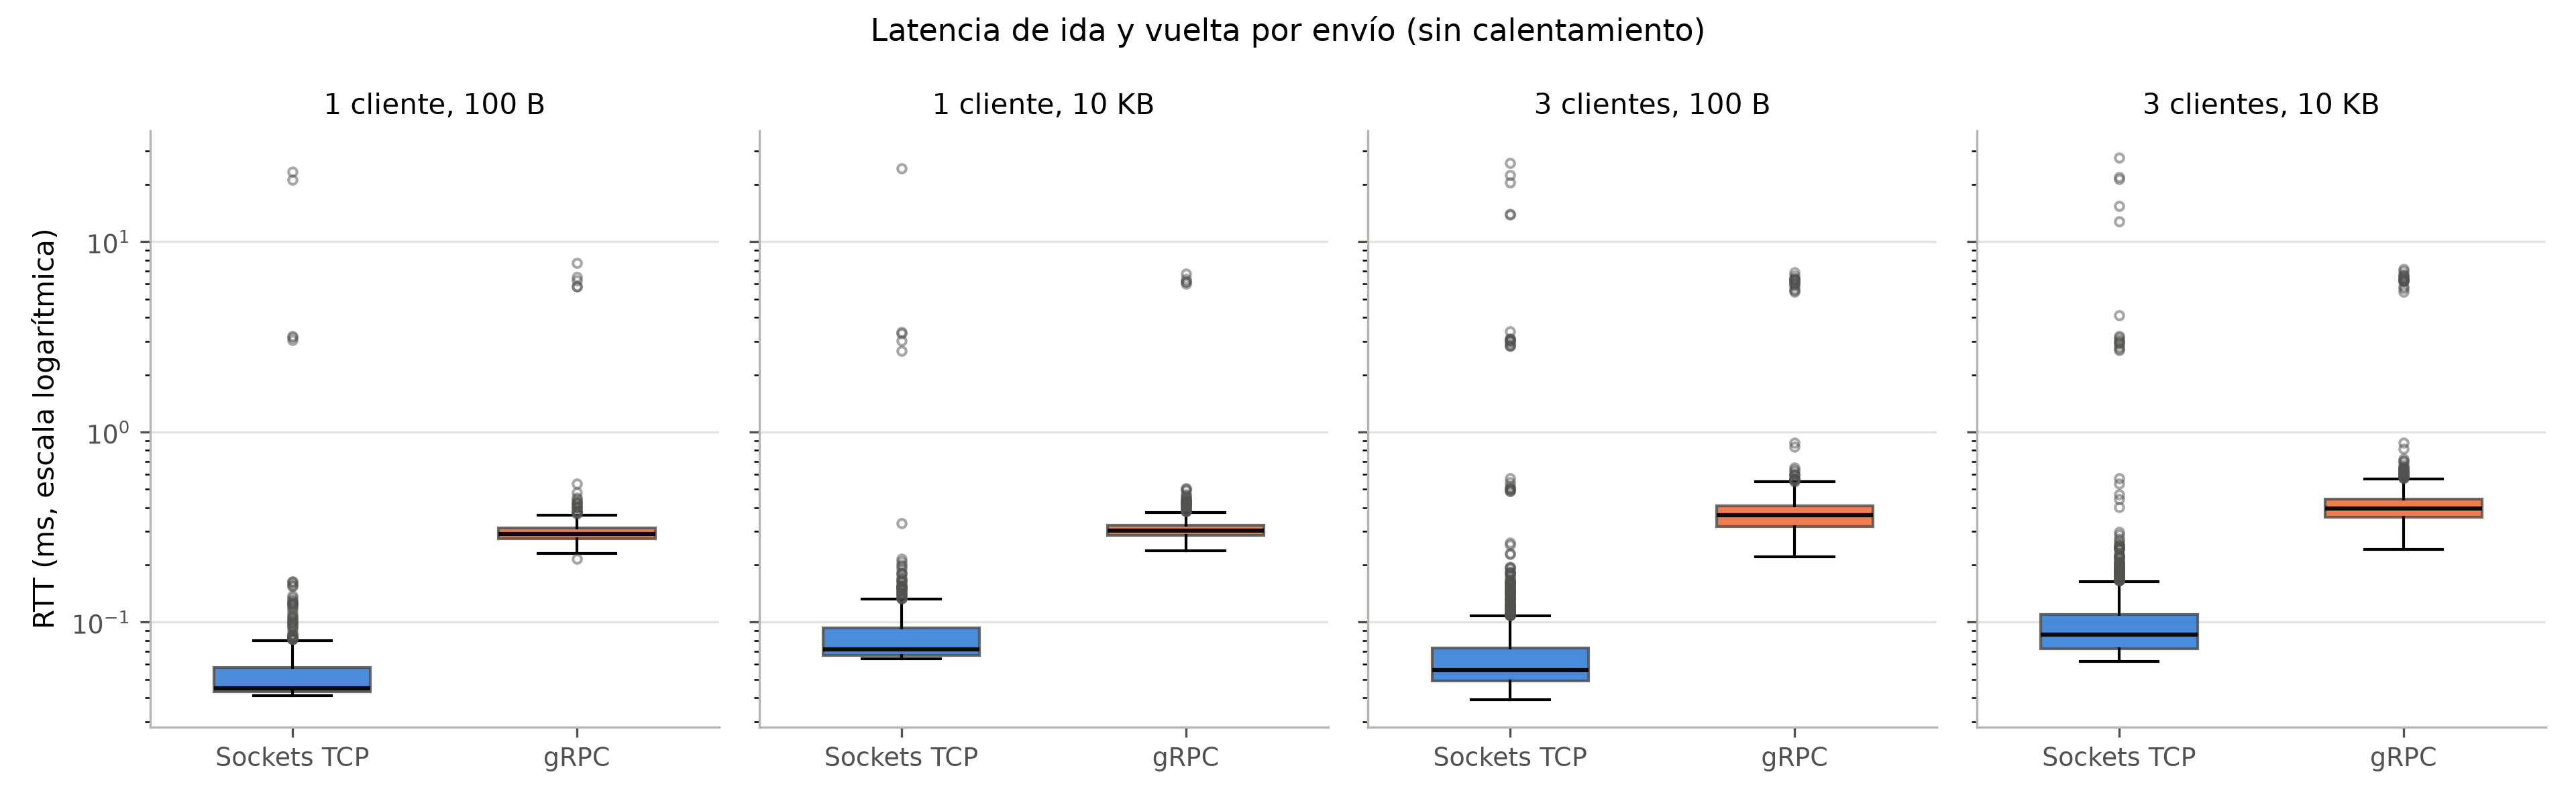
\includegraphics[width=\textwidth]{boxplot}
  \caption{Latencia de ida y vuelta de cada envío por condición, en escala logarítmica}
  \label{fig:boxplot}
\end{figure}

La Figura~\ref{fig:boxplot} muestra cómo se reparten los envíos. gRPC tiene una distribución estrecha, y su envío más lento tardó 7,8~ms. Sockets tiene la mediana más baja en las cuatro condiciones, pero 13 de sus 4000 envíos pasaron de 10~ms, con un máximo de 27,6~ms. Cuando uno de esos envíos cae en una repetición, alarga su duración, y por eso los mensajes por segundo de sockets cambian tanto de una repetición a otra: con un cliente y 100~bytes van de 3316 a 10\,850. Esa es la razón de que sus intervalos de confianza sean tan anchos en la Figura~\ref{fig:barras}. La mediana casi no se mueve con estos casos aislados.

\begin{figure}[htbp]
  \centering
  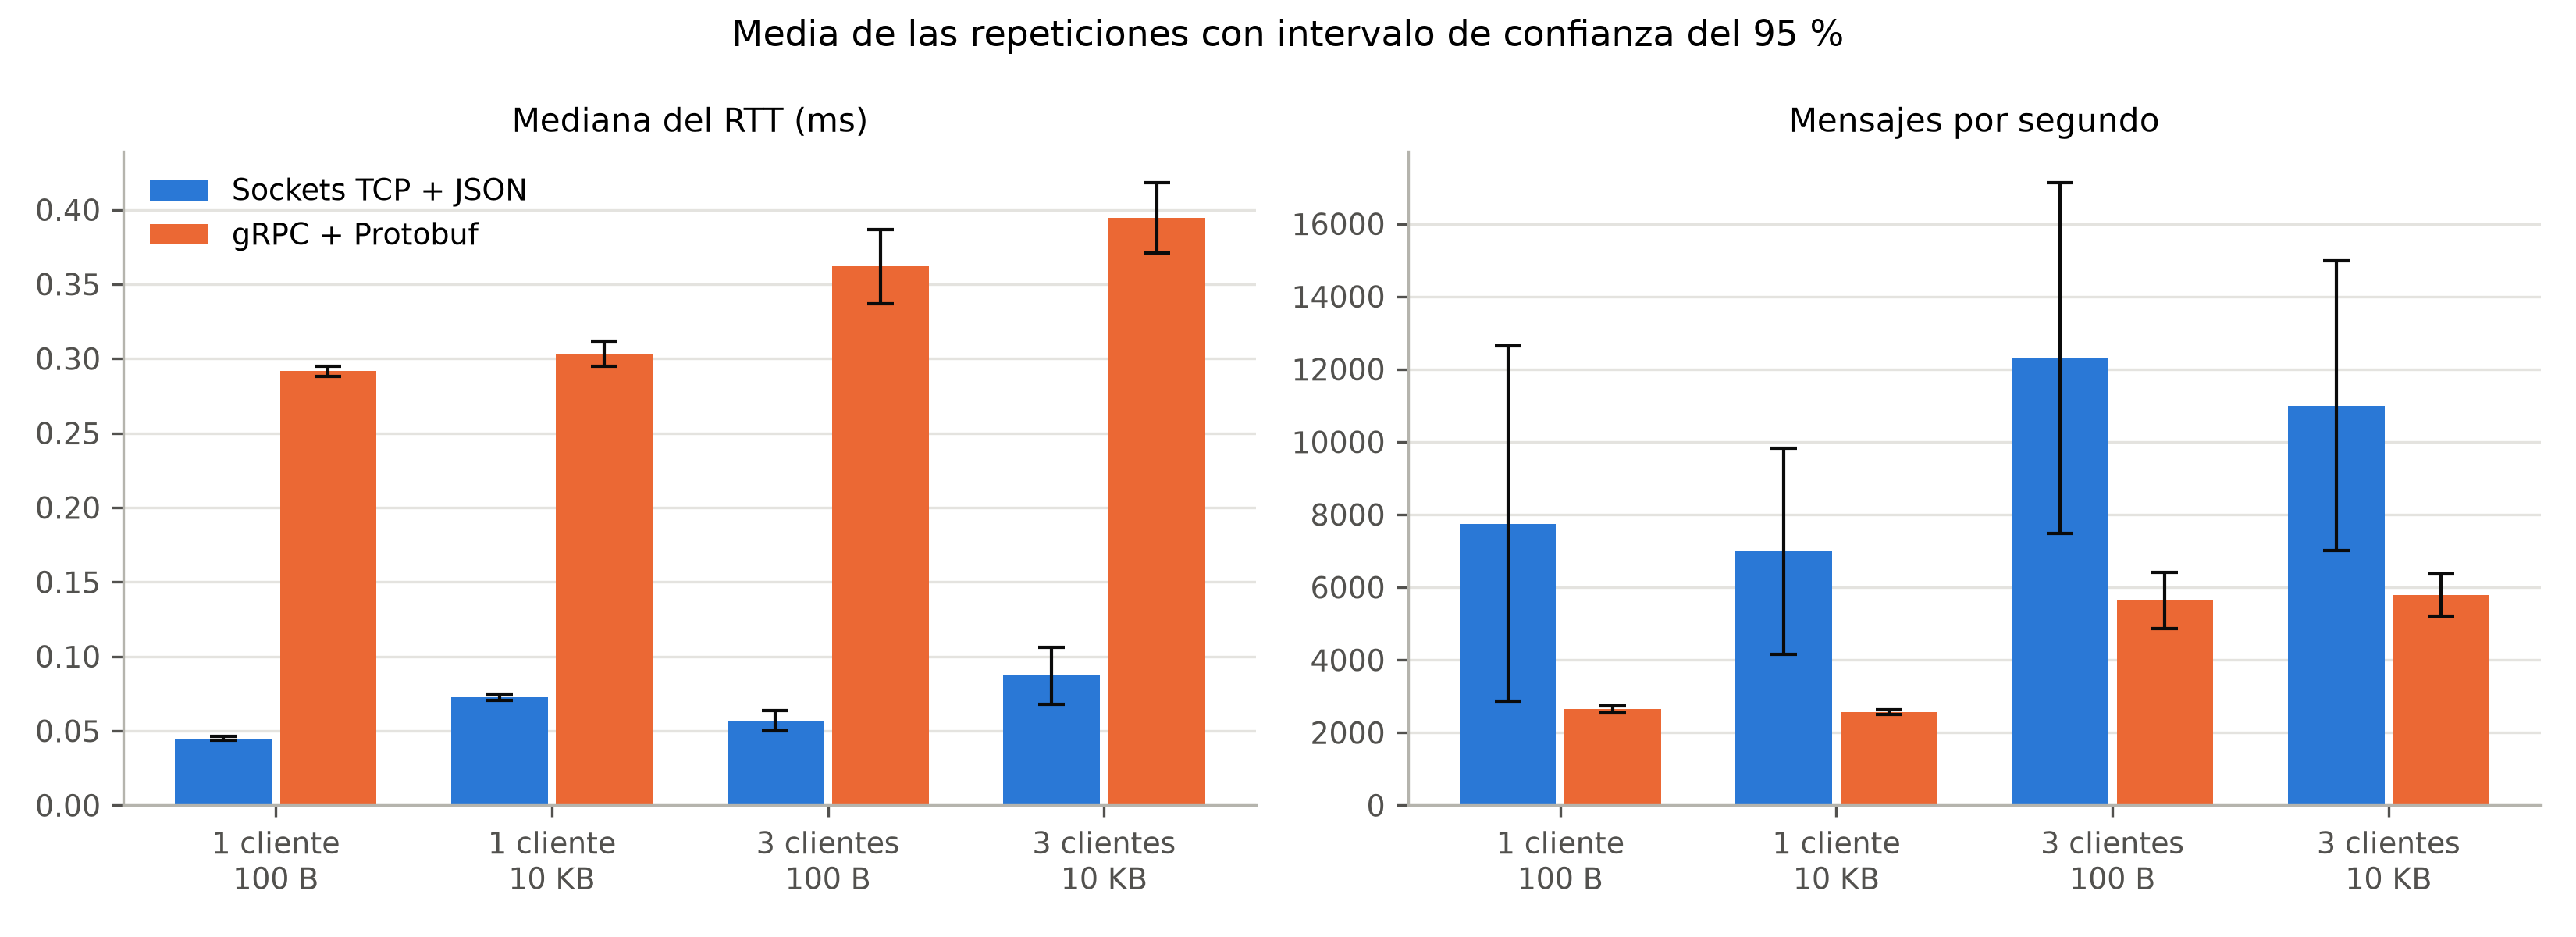
\includegraphics[width=\textwidth]{barras}
  \caption{Mediana del RTT y mensajes por segundo: media de las cinco repeticiones con intervalo de confianza del 95\,\%}
  \label{fig:barras}
\end{figure}

\subsection{Resultado de H1, H2 y H3}

\begin{table}[htbp]
  \centering
  \caption{Criterio de decisión aplicado a las hipótesis de latencia}
  \label{tab:hipotesis}
  \small
  % Generado por analysis/analizar.py. No editar a mano.
\begin{tabular}{>{\raggedright\arraybackslash}p{0.8cm} >{\raggedright\arraybackslash}p{2.6cm} >{\raggedright\arraybackslash}p{8.6cm} l}
\toprule
Hip. & Condición & Detalle & ¿Se cumple? \\
\midrule
H1 & 100 B, 1 cliente & mediana menor: sí; p95 menor: sí; más msg/s: sí & sí \\
H2 & 10 KB vs 100 B, 1 cliente & mediana menor con 10 KB: sí; cocientes 10 KB [3,97; 4,42] < cocientes 100 B [6,26; 6,85]: sí & sí \\
H3 & 100 B, 3 clientes vs 1 & mediana menor: sí; p95 menor: sí; cocientes 3 clientes [5,21; 7,49] > cocientes 1 cliente [6,26; 6,85]: no & no \\
\bottomrule
\end{tabular}

\end{table}

La Tabla~\ref{tab:hipotesis} aplica el criterio de la sección~1 a los valores de cada repetición. H1 se cumple: en la mediana, en el percentil~95 y en los mensajes por segundo, los rangos de las cinco repeticiones de los dos mecanismos no se traslapan. Incluso la peor repetición de sockets (3316 mensajes por segundo) supera a la mejor de gRPC (2737).

H2 también se cumple. Con 10~KB sockets mantiene menor mediana que gRPC, y los 25 cocientes entre las medianas de gRPC y de sockets con 10~KB (de 3,97 a 4,42) quedan todos por debajo de los 25 cocientes con 100~bytes (de 6,26 a 6,85).

H3 no se cumple. Con tres clientes, sockets tiene menor mediana y menor percentil~95 que gRPC, pero sus cocientes (de 5,21 a 7,49) se traslapan con los de un cliente. Con este criterio no se puede afirmar que la ventaja relativa de sockets haya crecido.

\subsection{Relojes de Lamport y convergencia}

En las 78 corridas se recibieron 20\,400 mensajes. En todos, el reloj de la recepción fue mayor que el del envío, y no quedó ningún envío sin su recepción. La verificación completa está en la sección de los relojes de Lamport.

\begin{table}[htbp]
  \centering
  \caption{Convergencia de los relojes de Lamport en las corridas de 20 intercambios}
  \label{tab:convergencia}
  \resizebox{\textwidth}{!}{% Generado por analysis/analizar.py desde analysis/lamport_convergencia.csv.
% No editar a mano.
\begin{tabular}{llrrrrrrr}
\toprule
Mecanismo & Nodos & Corridas & Convergen & Intercambios & Mín. (ms) & Mediana (ms) & Máx. (ms) & $>$100 ms \\
\midrule
Sockets TCP + JSON & 2 & 5 & 5 & 2 & 4,7 & 15,6 & 513,9 & 1 \\
Sockets TCP + JSON & 3 & 5 & 5 & 6 & 13,3 & 29,3 & 532,0 & 2 \\
Sockets TCP + JSON & 4 & 5 & 5 & 8 & 30,4 & 518,7 & 563,6 & 4 \\
gRPC + Protobuf & 2 & 5 & 5 & 2 & 5,6 & 5,7 & 6,3 & 0 \\
gRPC + Protobuf & 3 & 5 & 5 & 6 & 11,0 & 11,2 & 515,1 & 1 \\
gRPC + Protobuf & 4 & 5 & 5 & 8 & 11,6 & 13,0 & 21,9 & 0 \\
\bottomrule
\end{tabular}
}
\end{table}

Las 30 corridas de intercambios convergieron dentro de los 20 mensajes (Tabla~\ref{tab:convergencia}). El número de intercambios fue el mismo en todas las repeticiones de cada caso: 2 con dos nodos, 6 con tres y 8 con cuatro. Con los tiempos aparecen dos grupos. La mayoría de las corridas convergió entre 4,7 y 30,4~ms, pero 8 de las 30 tardaron más de medio segundo: 7 de sockets y 1 de gRPC. Las medianas con gRPC fueron 5,7, 11,2 y 13,0~ms para 2, 3 y 4 nodos; con sockets, 15,6, 29,3 y 518,7~ms.

Con el criterio de la sección~1, H4 no se cumple. El número de intercambios sí crece de 2 a 3 y a 4 nodos, pero no da 2, 4 y 6 como esperábamos. En el tiempo, los rangos se traslapan en los dos mecanismos; por ejemplo, una corrida de gRPC con 3 nodos tardó 515~ms, más que cualquiera de las de 4 nodos. La sección~\ref{sec:discusion-lamport} explica las dos cosas.


\section{Discusión}
\subsection{Por qué sockets fue más rápido}

H1 salió como esperábamos, y con una diferencia más grande de lo que pensábamos: con 100~bytes y un cliente, gRPC tardó unas 6,5 veces más que sockets en la mediana. En \emph{localhost} el paquete casi no viaja, así que esos 0,25~ms de más por mensaje salen del software. Con sockets, cada envío es un \texttt{json.dumps}, una línea por TCP y un \texttt{json.loads} del acuse. Con gRPC, cada llamada pasa además por las tramas y los encabezados de HTTP/2, los metadatos, el plazo de la llamada y el hilo del \texttt{ThreadPoolExecutor} que la atiende en el servidor. No medimos cada una de esas capas por separado, así que no podemos decir cuál pesa más. Lo que sí vemos es que el costo es fijo por llamada, porque se repite casi igual en las cinco repeticiones (de 0,288 a 0,295~ms).

Esto coincide con lo que reportan Zhu \emph{et al.}~\cite{Zhu2023}: en su medición, interpretar el protocolo de gRPC costaba bastante más que tratar el mismo tráfico como TCP. Y no contradice a Niswar \emph{et al.}~\cite{Niswar2024}, donde gRPC fue más rápido que REST y GraphQL, porque en ese estudio las otras opciones también pasaban por HTTP. Aquí sockets no tiene ninguna capa encima de TCP.

\subsection{Efecto del tamaño del mensaje}

H2 se cumplió, pero por un motivo distinto del que planteamos. Esperábamos que la diferencia en milisegundos se mantuviera y que pesara menos porque el total crecía en los dos mecanismos. La diferencia sí se mantuvo (de 0,25 a 0,23~ms), pero lo que bajó el cociente fue que sockets se hizo más lento con 10~KB (un 60\,\% más) y gRPC casi no cambió (un 4\,\% más). Creemos que la causa está en dónde se procesa el mensaje. En sockets, los 10~KB pasan por \texttt{json.dumps}, por la lectura de la línea y por \texttt{json.loads}, y parte de ese trabajo se hace en Python. En gRPC la serialización la hace la biblioteca de Protocol Buffers, cuya implementación para Python corre en código compilado. No lo comprobamos con un perfilador, así que lo dejamos como explicación probable. Lo que sí sale de los datos es que, en este rango de tamaños, el costo fijo de cada llamada de gRPC pesa mucho más que el costo de copiar 10~KB.

\subsection{Varios clientes a la vez}

H3 no se cumplió. Habíamos supuesto que con tres clientes gRPC sufriría más por el GIL, porque cada llamada pasa por más código Python de la biblioteca. Los datos no muestran eso: con 100~bytes, la mediana de sockets subió un 24\,\% y la de gRPC un 26\,\%, prácticamente lo mismo. Una posible explicación es que en gRPC la red y HTTP/2 los maneja el núcleo en C, que no necesita el GIL, y eso compensa el código Python extra. Por otro lado, la máquina tiene 28 hilos de procesador y los tres clientes son procesos separados, así que solo los servidores comparten el GIL.

Donde gRPC sí se acercó a sockets fue en los mensajes por segundo. Con tres clientes, gRPC atendió algo más del doble que con uno (de 2640 a 5636), y sockets un 59\,\% más (de 7747 a 12\,306). Aun así, sockets siguió atendiendo más mensajes por segundo en todas las condiciones. Este resultado hay que leerlo con cuidado, porque los mensajes por segundo de sockets varían mucho entre repeticiones.

\subsection{Los envíos lentos de sockets}

El resultado que no esperábamos es que sockets, con la mediana más baja, tenga los envíos más lentos de todo el experimento: 13 de 4000 pasaron de 10~ms y uno llegó a 27,6~ms, mientras que con gRPC ninguno pasó de 7,8~ms. Aparecen en 9 corridas distintas y en las cuatro condiciones, así que no vienen de una sola corrida que haya salido mal. No encontramos la causa; puede ser la planificación de hilos de Windows o algo del servidor de sockets, pero no lo medimos. Son el 0,3\,\% de los envíos, así que casi no mueven la mediana ni el percentil~95, pero sí la media y los mensajes por segundo. Por eso el criterio de decisión usa medianas y rangos por repetición, y no la media de todos los envíos. Si lo que importa es una latencia predecible, gRPC fue más estable en este experimento.

\subsection{Convergencia de los relojes de Lamport}
\label{sec:discusion-lamport}

El criterio de H4 decía que, si los intercambios no daban 2, 4 y 6, había que revisar la ronda antes de discutir la hipótesis. La revisamos. La hipótesis describe una ronda con una sola secuencia de mensajes: el primer nodo envía al segundo, este al tercero y así hasta volver al primero. Pero la ronda que quedó en el código el 20 de noviembre, antes de la corrida oficial, usa dos fichas que salen al mismo tiempo de dos nodos distintos. Así los dos primeros envíos son concurrentes, que es el caso que pide el enunciado. El camino que la información tiene que recorrer para llegar a todos es el mismo, pero mientras tanto la otra ficha también envía mensajes, y esos mensajes entran en la cuenta. Por eso salen 6 y 8 intercambios en vez de 4 y 6. Con dos nodos no cambia nada, porque basta con que cada uno reciba un mensaje del otro. No cambiamos la hipótesis después de ver los datos: la reportamos como estaba escrita y dejamos aquí la diferencia.

Lo que sí se mantiene es la tendencia. Los intercambios crecen de 2 a 6 y a 8, y siempre dan lo mismo en las cinco repeticiones, porque el patrón de envíos es fijo.

En el tiempo, H4 no se pudo confirmar por las 8 corridas que tardaron más de medio segundo. Revisamos una de ellas (sockets, 2 nodos, repetición~5). El nodo~A registró su primer envío y la recepción correspondiente en el otro nodo llegó 0,51~s después. Lo que pasó es que el nodo~A intentó conectarse antes de que el nodo~B abriera su puerto, y en Windows ese intento fallido tarda alrededor de medio segundo antes de que el nodo vuelva a intentar. Ese tiempo es arranque de los procesos y no convergencia de los relojes. Con gRPC, donde solo una corrida tuvo este problema, la tendencia sí se ve: las medianas son 5,7, 11,2 y 13,0~ms para 2, 3 y 4 nodos. Una corrección sería que los nodos esperen a que todos los servidores estén escuchando antes del primer envío. No repetimos la corrida con ese cambio, y lo dejamos como amenaza a la validez.

\subsection{Facilidad de desarrollo, tipado y manejo de errores}

\subsection{Amenazas a la validez}

En la discusión se explica cada una de estas amenazas; aquí solo las enumeramos con la forma de evitarlas.

\begin{itemize}
  \item Todo corrió en una sola máquina, en \emph{localhost}, sin red real. Para evitarlo habría que repetir el experimento en un entorno real, con los nodos en máquinas distintas de una red.
  \item 13 de los 4000 envíos de sockets pasaron de 10~ms (el máximo fue 27,6~ms) y no identificamos la causa. Ensanchan el intervalo de confianza de los mensajes por segundo. Lo evitaría cerrando procesos pesados en segundo plano durante la prueba, fijando la afinidad y prioridad de CPU de los nodos en el sistema operativo para evitar cambios de contexto bruscos, y haciendo más repeticiones para amortiguar picos aislados del planificador.
  \item 8 de las 30 corridas de Lamport tardaron cerca de 0,5~s en arrancar, porque un nodo intentó conectarse antes de que el otro abriera su puerto (sección~\ref{sec:discusion-lamport}). Para evitarlo, como se propone en la discusión, cada nodo debería esperar a que todos los servidores estén escuchando antes del primer envío. Ese cambio iría en \texttt{src/comun/nodo.py}.
  \item La ronda de dos fichas da 2, 6 y 8 intercambios, y la hipótesis esperaba 2, 4 y 6. Lo evitaría fijando primero el diseño exacto de la topología (si la ronda corre con una o con dos fichas simultáneas) antes de redactar la hipótesis, o calculando la predicción teórica de H4 directamente sobre el flujo real de mensajes de las dos fichas antes de ejecutar las corridas.
\end{itemize}


\section{Verificación de los relojes de Lamport}
% Sección 11 - Verificación de los relojes de Lamport (Dayver)
% Borra los comentarios cuando escribas el texto.

\subsection{Cómo se verificó}
% DATOS: el script analysis/verificar_lamport.py lee los 234 CSV de eventos
% (data/eventos_<mecanismo>_<nodo>_<equipo>_<corrida>.csv) de las 78 corridas.
% Empareja cada recepción con su envío: una recepción guarda en reloj_emisor el
% timestamp que traía el mensaje, así que su envío es la fila con
%   (corrida, nodo, reloj) del envío = (corrida, origen, reloj_emisor) de la recepción.
% Dentro de un nodo el reloj nunca se repite, por eso esa clave es única.
% Revisa: que toda recepción tenga su envío, que reloj de la recepción > reloj
% del envío, que todo envío tenga su recepción y que en cada nodo el reloj suba
% en cada fila. Verifica los datos reales: no genera valores.

\subsection{Resultado}
% DATOS (de analysis/lamport_resumen.csv y lamport_violaciones.csv):
% 20 400 recepciones en 78 corridas; las 20 400 cumplen reloj_recepcion >
% reloj_envio (100 %). Cero recepciones sin envío, cero envíos sin recepción,
% cero violaciones (lamport_violaciones.csv solo tiene el encabezado).
% Ojo: son 20 400 porque cuenta también las corridas de latencia (los nodos
% usan el reloj en todos los modos), no solo las 30 de intercambios.

\subsection{Dos eventos concurrentes con el mismo reloj}
% DATOS: corrida n3-r1 de sockets (CSV data/eventos_sockets_nodo-A_mcastro_n3-r1.csv
% y data/eventos_sockets_nodo-B_mcastro_n3-r1.csv):
%  - nodo-A: envío a nodo-B con reloj 1 (hora_real 1795365707.206059)
%  - nodo-B: envío a nodo-C con reloj 1 (hora_real 1795365707.207598)
%  Son los primeros eventos de cada nodo: ninguno había recibido nada, así que
%  ninguno pudo influir en el otro -> son concurrentes (a || b).
%  Por la hora real, A envió 1,5 ms antes que B, pero el reloj no lo refleja.
% POR QUÉ LAMPORT NO LOS DISTINGUE (explícalo tú):
%  - Lamport garantiza: si a -> b (a causa b), entonces C(a) < C(b).
%  - Lo contrario no vale: C(a) < C(b) no implica a -> b, y C(a) = C(b) no
%    dice cuál fue primero. Con el mismo valor solo se sabe que ninguno causó
%    al otro (si uno causara al otro, su reloj sería menor).
%  - Es un solo número por evento: no guarda de qué nodos viene la información.
%    Para distinguir concurrencia de causalidad se necesitan relojes vectoriales.
%  - Para un orden total se desempata con el nombre del nodo (A antes que B),
%    pero ese orden es una convención, no lo que pasó.

\subsection{Convergencia}
% DATOS: no repitas la tabla. Refiere la de la sección 7: \ref{tab:convergencia}.
% Las 30 corridas convergen; 2, 6 y 8 intercambios con 2, 3 y 4 nodos, con
% reloj 2, 6 y 8 en todas las repeticiones, porque cada nodo recibe de un solo
% antecesor por una sola conexión y el orden de los eventos siempre es el mismo.
% El tiempo sí varía; la explicación está en \ref{sec:discusion-lamport}.


\section{Conclusiones}
En tres nodos en \emph{localhost}, con Python~3.13 y una conexión o un canal por cliente, sockets TCP con JSON tuvo menor latencia que gRPC con Protocol Buffers en las cuatro condiciones que medimos. Con 100~bytes y un cliente, la mediana fue de 0,045~ms frente a 0,291~ms, y sockets atendió unos 7700 mensajes por segundo frente a 2600 de gRPC. H1 se cumple: la diferencia está en cada repetición y los rangos de los dos mecanismos no se tocan.

El tamaño del mensaje redujo la ventaja relativa de sockets, como decía H2. Con 10~KB, gRPC tardó unas 4,2 veces más que sockets, frente a 6,5 veces con 100~bytes. Eso pasó porque sockets se hizo más lento con el mensaje grande y gRPC casi no cambió. La diferencia en milisegundos se quedó cerca de 0,23~ms. En estos tamaños, lo que más cuesta en gRPC es el trabajo fijo de cada llamada, no el contenido.

H3 no se confirmó. Con tres clientes a la vez, las medianas de los dos mecanismos subieron en proporción parecida, y no se puede decir que la ventaja de sockets haya crecido. gRPC aprovechó mejor la concurrencia en mensajes por segundo (los duplicó, mientras que sockets los subió un 59\,\%), aunque sockets siguió por encima.

gRPC fue más estable. Su envío más lento tardó 7,8~ms, mientras que sockets tuvo 13 envíos de más de 10~ms, cuya causa no identificamos. Para este caso, sockets es la opción con menos latencia; si se necesita que el tiempo de respuesta sea predecible, los datos favorecen a gRPC. La facilidad de desarrollo de cada mecanismo se trata en la sección de discusión y no cambia estos números.

Los relojes de Lamport funcionaron con los dos mecanismos: en los 20\,400 mensajes, el reloj de la recepción fue mayor que el del envío. La convergencia necesitó 2, 6 y 8 intercambios con 2, 3 y 4 nodos. El número crece con los nodos, pero no da los valores que pusimos en H4, porque la ronda final usa dos fichas y la hipótesis suponía una. En el tiempo, H4 no se confirmó porque algunas corridas incluyen medio segundo de arranque de los procesos.

Todo esto se midió en una sola máquina y sin red real. Con una red de verdad, el tiempo de transmisión se sumaría a los dos mecanismos, y esperamos que la diferencia relativa sea menor. Para repetir el experimento conviene que los nodos esperen a que todos los servidores estén escuchando antes del primer envío, y buscar la causa de los envíos lentos de sockets.

\subsection{Conclusiones individuales}

% Cada integrante escribe aquí su propia conclusión (mínimo 150 palabras):
% qué aprendió, qué le costó, qué haría distinto. Borrar la línea "Pendiente" al escribirla.

\subsubsection*{Castro Coello Mario Sebastián}
\textit{Pendiente.}

\subsubsection*{Loor Suárez Steffanny del Rocío}
Durante esta práctica pude comprender mejor cómo funciona la
comunicación entre procesos mediante sockets TCP y cómo
se relaciona con los sistemas distribuidos.
Mi participación en esta tarea se centró en desarrollar el servidor y
el cliente TCP, comprobar el intercambio de mensajes e
integrar esta comunicación con el reloj lógico de Lamport.
Con ello entendí que no basta con enviar información,
sino que también es necesario validar los datos y confirmar su
recepción y controlar las conexiones.

Una de las dificultades que encontré fue conseguir que los
procesos se comunicaran correctamente y manejar los errores
que podían aparecer cuando un nodo todavía no estaba disponible.
También tuve que revisar el funcionamiento de los mensajes de
confirmación y comprobar que la integración con el reloj de Lamport
mantuviera el orden lógico de los eventos.

Puedo dar como conclusión de esta práctica que según los resultados
TCP puede ofrecer una latencia menor que gRPC en las condiciones
evaluadas, aunque eso no significa que siempre sea la mejor alternativa.
Si volviera a realizar esta práctica, organizaría desde el inicio pruebas
más específicas para detectar los errores de conexión y verificaría
que todos los servidores estuvieran preparados antes de comenzar los intercambios.

\subsubsection*{Quintero Rico Luis David}
\textit{Pendiente.}

\subsubsection*{Rivas Piloso Dayver Yahir}
\textit{Pendiente.}


\section{Aportes de los integrantes}
Cada integrante trabajó en su propia rama y entró a \texttt{main} por un \emph{pull request} revisado. Los enlaces llevan al commit en el repositorio; el detalle de cada día está en \texttt{BITACORA.md}.

\newcommand{\commit}[1]{\href{https://github.com/reyshadow0/isr701-pe-u1/commit/#1}{\texttt{#1}}}

{\footnotesize
\begin{longtable}{@{}>{\raggedright\arraybackslash}p{2.8cm}>{\raggedright\arraybackslash}p{7.3cm}>{\raggedright\arraybackslash}p{4.9cm}@{}}
  \caption{Aportes de cada integrante y sus commits}
  \label{tab:aportes} \\
  \toprule
  \textbf{Integrante} & \textbf{Aporte} & \textbf{Commits} \\
  \midrule
  \endfirsthead
  \toprule
  \textbf{Integrante} & \textbf{Aporte} & \textbf{Commits} \\
  \midrule
  \endhead
  Castro Coello Mario Sebastián &
  Estructura del repositorio, plan de trabajo y bitácora. Reloj de Lamport con \texttt{threading.Lock} (\texttt{src/comun/lamport.py}) y sus pruebas. Objetivo, hipótesis y criterio de decisión. Revisión y fusión de los \emph{pull requests}. Corrida oficial en su equipo, datos crudos con \texttt{SHA256SUMS}, script de análisis (\texttt{analysis/analizar.py}), evidencias, y las secciones de resultados, discusión y conclusiones. &
  \commit{7a14cc6}, \commit{b6438e6}, \commit{aa1a600}, \commit{5e93693}, \commit{36e9064}, \commit{caf1204}, \commit{0b6c1e9}, \commit{154943b}, \commit{3a66697}, \commit{0ec97b3} \\
  \midrule
  Loor Suárez Steffanny del Rocío &
  Servidor y cliente TCP con mensajes JSON por línea, acuses y una conexión por destino (\texttt{src/sockets/}). Integración con la interfaz común y el reloj de Lamport. Primeras mediciones de latencia y evidencias de los tres nodos TCP. Diagrama de la arquitectura. &
  \commit{27fea0b}, \commit{d7a7f0f}, \commit{12fbe7b}, \commit{8ca71bf}, \commit{109ca32} \\
  \midrule
  Quintero Rico Luis David &
  Contrato del servicio en \texttt{proto/messaging.proto}, código generado, servidor y cliente gRPC con un canal por destino (\texttt{src/grpc/}). Integración con la interfaz común. Secciones del contrato, de gRPC y de facilidad de desarrollo. &
  \commit{382427e}, \commit{6e61741} \\
  \midrule
  Rivas Piloso Dayver Yahir &
  \texttt{requirements.txt} y registro de las condiciones de la máquina (\texttt{src/experimento/condiciones.py}). Script que corre el protocolo completo (\texttt{correr\_experimento.py}), lógica común de los nodos (\texttt{src/comun/nodo.py}) y verificador de Lamport con el cálculo de convergencia (\texttt{analysis/verificar\_lamport.py}), con sus pruebas. Secciones de protocolo, amenazas a la validez y verificación de Lamport. &
  \commit{ed71bbd}, \commit{9c28faf}, \commit{ef37a8f}, \commit{e999845}, \commit{f6916bc}, \commit{ed992d7}, \commit{1401826} \\
  \bottomrule
\end{longtable}
}


\section{Declaración de uso de inteligencia artificial}
{\footnotesize
\begin{longtable}{@{}>{\raggedright\arraybackslash}p{2.2cm}>{\raggedright\arraybackslash}p{2.2cm}>{\raggedright\arraybackslash}p{1.6cm}>{\raggedright\arraybackslash}p{3.9cm}>{\raggedright\arraybackslash}p{3.9cm}@{}}
  \caption{Herramientas de inteligencia artificial usadas como apoyo}
  \label{tab:declaracion-ia} \\
  \toprule
  \textbf{Integrante} & \textbf{Herramienta} & \textbf{Versión} & \textbf{Para qué se usó} & \textbf{Cómo se verificó lo obtenido} \\
  \midrule
  \endfirsthead
  \toprule
  \textbf{Integrante} & \textbf{Herramienta} & \textbf{Versión} & \textbf{Para qué se usó} & \textbf{Cómo se verificó lo obtenido} \\
  \midrule
  \endhead
  Castro Coello Mario Sebastián & Claude Code & Opus 5.5 & 18/11: proponer el reparto y el plan por día, redactar los mensajes al grupo, armar el esqueleto del repositorio, las ramas y la plantilla de la bitácora, y explicar el reloj de Lamport y \texttt{threading.Lock}. & El reparto se decidió en grupo y los tres integrantes lo aceptaron. El commit y el push los hizo Mario. \\
  \midrule
  Castro Coello Mario Sebastián & Claude (chat) y Claude Code & Opus 5.5 & 20/11: revisar las tres versiones de \texttt{lamport.py}; encontró tres problemas y metió 8 errores a propósito para comprobar las pruebas. & Mario corrió las 9 pruebas en su PC; la versión final las pasa y las pruebas detectan los 8 errores. \\
  \midrule
  Castro Coello Mario Sebastián & Claude (app conectada al repositorio) & Opus 5.5 & 22/11: escribir \texttt{analysis/analizar.py} y guiar los comandos de la corrida oficial, del \texttt{SHA256SUMS} y de las capturas. & Mario ejecutó todo en su equipo: 78 corridas en \texttt{ok}, \texttt{SHA256SUMS} comprobado (336 archivos) y salidas del análisis revisadas contra el criterio de la sección~1. \\
  \midrule
  Castro Coello Mario Sebastián & Claude (app conectada al repositorio) & Opus 5.5 & 22/11: revisar los datos; encontró que el análisis contaba las corridas de prueba, que la ronda con dos fichas da 2, 6 y 8 intercambios y los 0,5~s de arranque en Lamport. & Mario revisó los CSV y los registros de la corrida \texttt{n2-r5}; la hipótesis se dejó como estaba escrita. \\
  \midrule
  Castro Coello Mario Sebastián & Claude (app conectada al repositorio) & Opus 5.5 & 22/11: buscar referencias candidatas con DOI para la discusión. & Datos bajados con \texttt{doi2bib.ps1} y contrastados con el script \texttt{verificar-\allowbreak referencias.ps1}; Mario leyó los resúmenes de las obras citadas. \\
  \midrule
  Loor Suárez Steffanny del Rocío & ChatGPT (web) & GPT-6 & 19/11: sugerencias para mejorar el servidor TCP (atención con hilos y validación de tipos). & Incorporó los cambios a mano y probó el servidor con mensajes válidos e inválidos en su PC. \\
  \midrule
  Loor Suárez Steffanny del Rocío & ChatGPT (web) & GPT-6 & 20/11: revisar las observaciones del \emph{pull request} (tiempo de espera en \texttt{accept()} y orden del acuse). & Probó Ctrl+C, el acuse y 10 clientes a la vez en PowerShell. \\
  \midrule
  Loor Suárez Steffanny del Rocío & ChatGPT (web) & GPT-6 & 21/11: orientación para integrar cliente y servidor TCP con la interfaz común y analizar errores de conexión. & Corrió tres nodos con 20 intercambios y el verificador de Lamport (100\,\% de recepciones válidas). \\
  \midrule
  Quintero Rico Luis David & ChatGPT & GPT-6 & 19/11: resolvio la instalación, genero una base del servidor y cliente gRPC y de esta manera podee entender su funcionamiento. & Generó los módulos del \texttt{.proto}, revisó las importaciones y probó la comunicación entre los dos terminales en vs code. \\
  \midrule
  Quintero Rico Luis David & ChatGPT & GPT-6 & 22/11: brindo apoyo para integrar gRPC con \texttt{NodoComun}, revisar el cliente y el servidor. &
Ejecuté las 40 pruebas unitarias y las pruebas locales del experimento apoyandome tambien con el analisis de los resultados obtenidos en las pruebas para las conclusiones.\\
  \midrule
  Rivas Piloso Dayver Yahir & Claude & Opus 5.5 & 18/11: comandos de instalación en Windows y estructura de \texttt{condiciones.py}. & Instaló el entorno, ejecutó el script y comprobó que los datos coincidieran con su equipo. \\
  \midrule
  Rivas Piloso Dayver Yahir & Claude & Opus 5.5 & 20/11: estructurar \texttt{correr\_experimento.py}, \texttt{verificar\_lamport.py}, \texttt{src/comun/nodo.py} y sus pruebas. & Probó el flujo con un nodo simulado y pruebas de hilos en memoria, y corrió las 24 pruebas del repositorio. \\
  \bottomrule
\end{longtable}
}


\printbibliography[heading=bibintoc,title={Referencias}]

\end{document}
